\chapter{Umsetzung - Jordi}
\label{\docname}

\section{Allgemeine Beschreibung}
Ein wichtiger Teil jedes Projekt ist die Datenbank, und dass ist der Teil wo ich am meisten konzentriert bin. Andere Teilebereiche wo ich teilnehmen habe, sind bei der Extraktion der Gesichtspunkte, wo mein Job, den Tiefe von Bildern zu finden, damit ein 2D vs. 3D unterschied geben sollte, ist.

\begin{table}[ht]
	\centering
	\begin{tabular}{ |l|l|l| } 
		\hline		
		Technologie & Beschreibung & Lizenz \\ 
		\hline
		MySQL & Datenbankverwaltungssystem & Kostenlos \\ 
		\hline
		MariaDB & Datenbankverwaltungssystem & Kostenlos \\
		\hline 
		Python & Objekte-orientierte Programmiersprache & Kostenlos \\
		\hline 
		OpenCV &  Bildverarbeitung Programmbibliothek  & Kostenlos \\ 
		\hline
	\end{tabular}
	\caption{Technologien}
	\label{table:tech}
\end{table}
\subsubsection{MySQL}
\begin{figure}
	\centering
	
\includegraphics[scale=0.3]{./figures/mysql.jpg}
	\caption{ MySQL Logo}
	\label{fig:mysql}
	\cite{MySQLlogo}
\end{figure}
MySQL ist eine echte Multi-User, Multi-Treaded SQL Datenbank und wird von allen großen
Providern oder auch Suchmaschinenbetreibern eingesetzt. MySQL ist eine CLient/Server
Implentierung, die aus einem Server-Dämon mysqld und vielen Client Programmen, sowie
Bibliotheken für PERL, PHP/3, PHP/4 sowie ASP besteht.
SQL ist eine standardisierte Datenbanksprache, die das Speichern, Updaten und den Zugriff auf
Informationen erleichtert. Beispielsweise kann man Produktinformationen eines Kunden auf einem
WWW-Server speichern und abrufen. MySQL ist äußerst schnell und flexibel genug, um sogar Bilder
und Log-Dateien darin abzulegen. In der Praxis ist MySQL sehr viel schneller, als z.B. ORACLE oder INFORMIX.\cite{stepken1999mysql}
\bigbreak
MySQL hat ein breites Anwendungsspektrum und wird meistens in Verbindung mit PHP, Linux, Python usw. verwendet. Der Grund zu der Auswahl von MySQL steht bei der einfachen Bedienung und Verwaltung von Datenbank. Da es sich bei DBS um eines der am häufigsten verwendeten DBS handelt, gibt es eine Vielzahl von Tools, die zum Verwalten der Datenbank verwendet werden können.

\subsubsection{MariaDB}
MariaDB ist aktuell die am schnellsten wachsende Open-Source-Datenbanklösung. Sie wird hauptsächlich von der MariaDB Corporation entwickelt und ist ein Fork von MySQL. Mittlerweile bietet das Datenbankverwaltungssystem mit seinen diversen kostenfreien Features vieles, was MySQL nicht oder nur kostenpflichtig zur Verfügung stellt (z.B. eine Speicher-Engine zur performanten Verarbeitung von riesigen Datenmengen; ein Datenbank-Proxy zur sicheren und hoch-verfügbaren Verwaltung skalierbarer Installationen u.v.m.). Im Gegensatz zu MySQL verfügt MariaDB jedoch nicht über einen eigenen Client wie die Workbench. Eine gute kostenfreie Alternative stellt HeidiSQL dar, jedoch verfügt diese über kein Dashboard, welches z.B. die Funktionsweise des Servers darstellt und damit Optimierungsentscheidungen erleichtert.\cite{MariaDB-Monitor}
\begin{figure}[h]
	\centering
	
\includegraphics[scale=0.3]{./figures/mariadb.png}
	\caption{ MariaDB Logo}
	\label{fig:mariadb}
	\cite{MariaDBlogo}
\end{figure}
\bigbreak
Es ist hauptsächlich in Linux implementiert, da es das Standard-DBS ist. Es bietet eine einfache Verbindung mit Linux-Dateien wie Python, C ++ und vielen anderen Programmiersprachen. Da dies der Standard-Linux-DBS ist und unsere Software unter Linux mit Python-Skripten geschrieben wurde, ist MariaDB unsere Wahl für DBS.

\subsubsection{Python}
Python ist eine Programmiersprache, die dank ihrer klaren Syntax und einfachen Lesbarkeit leicht zu erlernen ist und sich sehr vielseitig einsetzen lässt. Für die gängigen Betriebssysteme ist Python frei verfügbar. Die üblichen Programmierparadigmen wie die objektorientierte oder funktionale Programmierung werden unterstützt.\\
Bei Python handelt es sich um eine Programmiersprache mit einer klaren Syntax und guten Lesbarkeit. Sie gilt als leicht zu erlernen und ist in den gängigen Betriebssystemen interpretierbar.Python unterstützt mehrere Paradigmen der Programmierung wie die funktionale, objektorientierte oder aspektorientierte Programmierung und ist auch als Skriptsprache nutzbar.\cite{pythonInfo}
\begin{figure}[ht]
	\centering
	
\includegraphics[scale=0.3]{./figures/python.png}
	\caption{ Python Logo}
	\label{fig:python}
	\cite{Pythonlogo}
\end{figure}
 Die Sprache weist ein offenes, gemeinschaftsbasiertes Entwicklungsmodell auf, das durch die gemeinnützige Python Software Foundation gestützt wird, die de facto die Definition der Sprache in der Referenzumsetzung CPython pflegt.

\bigbreak
Der Grund, warum die Software in Python geschrieben ist, ist, dass Python eine einfache und schnelle Möglichkeit bietet, Datenbankskripte und Gesichtserkennungsprogramme zu erstellen.
\subsubsection{OpenCV}
OpenCV (Open Source Computer Library) ist eine Open-Source-Bibliothek für Computer Vision und Machine-Learning-Software. OpenCV wurde entwickelt, um eine gemeinsame Infrastruktur für Computer Vision-Anwendungen bereitzustellen und die Nutzung der maschinellen Wahrnehmung in den kommerziellen Produkten zu beschleunigen. Als BSD-lizenziertes Produkt macht OpenCV es Unternehmen leicht, den Code zu nutzen und zu ändern.Es verfügt über C++, Python, Java und MATLAB-Schnittstellen und unterstützt Windows, Linux, Android und Mac OS.\cite{OpenCV}
\begin{figure}[ht]
	\centering
	
\includegraphics[scale=0.3]{./figures/opencv.png}
	\caption{ OpenCV Logo}
	\label{fig:opencv}
	\cite{OpenCVlogo}
\end{figure}
\bigbreak
Obwohl es in C ++ geschrieben wurde, bietet es viele Schnittstellen zu anderen Programmiersprachen wie Python, die in diesem Projekt implementiert werden. OpenCV ist eine plattformübergreifende Bibliothek und da es viele Deep-Learning-Algorithmen und Frameworks enthält, musste es unsere Wahl für die Objekterkennung sein.
\section{Technische Lösungen}
\subsection{Datenkbank}
Wie bereits erwähnt, haben wir uns für MySQL und MariaDB als DBS entschieden, wobei meistens das zweite mehr zum Einsatz kommt. Es ist wichtig zu beachten, dass die Datenbank nicht über die Befehlszeile oder die MySQL/MariaDB-Konsole implementiert wurde, sondern mithilfe von Python-Skripten. In diesem Fall würde jeder gegebene Befehl in den Python-Dateien gespeichert, und wenn etwas schief ging, könnten die Skripte einfach verbessert und ein Fehler behoben werden.
\bigbreak
Um eine Datenbank zur Gesichtserkennung und -identifikation zu entwerfen, mussten einige Nachforschungen angestellt werden, bei denen es hauptsächlich darum ging, Beispiele für vorhandene Datenbanken zu finden. Auf diese Weise könnten wir uns eine Vorstellung davon machen, wie die Datenbanken aussehen. Obwohl die meisten Datenbanken nicht kostenlos waren und einige Unterlagen unterschrieben werden mussten, um die vollständigen Details zu erhalten, war dies mehr als ausreichend, um einen Ausgangspunkt zu haben. Einige der gefundenen Datenbanken sind:
\begin{itemize}
	\item 3D Mask Attack Dataset
	\item The AR Face Database, The Ohio State University
	\item Caltech Faces
	\item CAS-PEAL Face Database
	\item The Color FERET Database, USA
\end{itemize}
Auf den ersten Blick scheint es nicht sehr schwierig zu sein, eine Gesichtserkennungsdatenbank zu erstellen, aber da sich das Projekt entwickelt, müssen viele Änderungen vorgenommen werden, da sie an die Gesichtsdaten der Person weitergegeben werden müssen.
\bigbreak
Der nächste Schritt bestand darin, in Python nachzuforschen, wie die Schnittstelle mit MariaDB verbunden wird. Da es von vielen Linux-Benutzern empfohlen wurde, Python als beste Wahl für die Verbindung zu MariaDB zu wählen, wurde der Programmierer aufgefordert, den Code mithilfe von Methoden und try and except-Anweisungen zu schreiben, um einige saubere und perfekte Skripte zu erstellen. Auf diese Weise wäre der Code sehr einfach zu analysieren und zu verbessern, aber am wichtigsten wäre es, Fehlermeldungen zu beseitigen.
\subsubsection{Beschreibung der Tabellen}
Nach der anfangs Planung wurden drei Tabellen definiert, die folgenden Tabellen:
\begin{itemize}
	\item Person
	\item Info
	\item Log
\end{itemize}
\subsubsection{Tabelle Person}
Die erste Tabelle, Person, enthält alle User mit ihren grundlegenden Informationen, wie Vorname, Nachname, Rolle, Email. Die Spalte Rolle ist damit geeignet, damit ein Unterschied zwischen Personen geben sollte, weil es zwei Gruppen, die Admins und des normalen Users. Die Admin bekommen die Zahl 1 bei der Rolle, wahrend die anderen Users 0. Bei den Spalten, wo der Datentyp varchar verwendet wurde, gibt es ein Grund wiese varchar und nicht char. Das ist so denn char den ganzen Platzt reserviert, wo anderseits der Datentyp varchar nur die Lange des gespeicherten Strings reserviert, obwohl die Spalte ein varchar mit der Lange 50 sein kann.
\bigbreak
Die Spalte idP ist eine eindeutige Spalte, die es zu der Identifizierung von der Datenzeile gilt, deshalb wird auch als Primar Schlüssel definiert. Es wird auch auto increment festgelegt, damit die nächste Zeile automatisch die nächste Zahl bekommt.
\bigbreak
Die Spalte Nachname enthält der Nachname der Person, deshalb wird als Datentyp Varchar mit der Lange 50 gespeichert, weil Varchar zum Speichern von Strings geeignet ist.
bekommt.
\bigbreak
Die Spalte Email enthält der Email der Person, deshalb wird als Datentyp Varchar mit der Lange 50 gespeichert, weil Varchar zum Speichern von Strings geeignet ist.
bekommt.
\bigbreak
Die Spalte Rolle enthält der Rolle der Person, deshalb wird als Datentyp Char mit der Lange 1 gespeichert, weil Char zum Speichern von Strings geeignet ist. Um eine einfache Nummer zu speichern, ist hier auch den Datentyp int verwendbar.

\subsubsection{Tabelle Info}
Die zweite Tabelle enthält die Bilder der Personen, die wahrend der Zeit gemacht wurden, und auch die Grund Information der Bilder, wie Punkten und der Path von dem Bild. Die Spalten der folgenden Tabellen sind:
\bigbreak
Die Spalte idF ist eine eindeutige Spalte, die es zu der Identifizierung von der Datenzeile gilt, deshalb wird auch als Primar Schlüssel definiert. Es wird auch auto increment festgelegt, damit die nächste Zeile automatisch die nächste Zahl bekommt.
\bigbreak
Die Spalte idP ein fremder Schlüssel, der als Primar Schlüssel für die Person Tabelle geeignet ist. Diese fremden Schlüssel sind dazu, damit eine Verbindung zwischen diese zwei Tabellen geben kann. Diese zwei Tabelle haben eine 1 zu mehreren Beziehungen, wo eine Person mehrere Bilder haben kann. Das wurde so geplant, damit je mehr Bilder eine Person hat, desto sicher, besser und funktionierbar der Vergleich sein kann.
\bigbreak
Jeder Punkt besteht aus eine X und Y Koordinate, und von jedem Bild gibt es einen Startpunkt, wo die anderen Punkten relativ zu diesem Punkt gespeichert werden. Für diese Punkte wird den Datentyp dezimal werden, weil die Koordinaten kommastellen Zahlen sind. Nur für den ersten Punkt werden genau die Koordinaten gespeichert, für die anderen zeigt die X- und Y- Koordinate einen Vektor, das heißt es wird der Distanz von diesem Startpunkt aufgenommen.
\bigbreak
Die Spalte imagePath speichert die Path der Bilder und wird mit dem Datentyp varchar mit einer Länge von 50 gespeichert, weil Varchar zum Speichern von Strings geeignet ist. Die Bilder wurden als Path und nicht als ganze Image gespeichert, weil ob diese Bilder in der Datenbank gespeichert werden, wurde die Datenbank überfüllt mit Daten. Alternativ was medium blob aber dieser Datentyp brauch zu viel Speicherplatz von unserer Datenbank. Es konnte eine Overflow von der Datenbank geben.

\subsubsection{Log Tabelle}
Die dritte Tabelle ist nichts anders als eine Tabelle, wo alle Änderungen in der Datenbank protokoliert werden. In diesen Tabellen sollten die Grund Informationen gespeichert werden müssen, wie z.B wer hat was, wann gemacht. Diese frage muss die Tabelle beantwortet.
\bigbreak
Die Spalte idL ist eine eindeutige Spalte, die es zu der Identifizierung von der Datenzeile gilt, deshalb wird auch als Primar Schlüssel definiert. Es wird auch auto increment festgelegt, damit die nächste Zeile automatisch die nächste Zahl bekommt.
\bigbreak
Die Spaltet User soll der Person speichert, wer die Änderungen durchgeführt hat. Hier wird der Datenbank User gespeichert, weil um etwas zu verändern soll die Person zuerst in der Datenbank einloggen. Die Spalte hat den Datentyp Varchar mit der Lange 50, weil die Funktion Current User, da eingetragen wird.
\bigbreak
Die Spalte Date als der Name zeigt, kümmert um die Speicherung von der Zeit, wann eine SQL Statement ausgeführt wird. Die Spalte hat den Datentyp datetime, und da wird die Funktion now(), die die aktuelle Zeit darstellt, gespeichert.
\bigbreak
Die Spalte Info, informiert den User, was für eine Änderung gemacht wurde, z.B neue User wurde eingelegt. Diese Spalte bekommet den Datentyp Varchar, weil Varchar zum Speichern von Strings geeignet ist. Die Werten in dieser Spalte werden durch Triggers definiert, also wenn etwas in der Datenbank passiert, kümmern die Triggers um die eintragen von Daten.
\newpage
\section{Herausforderungen}
Jedes Projekt hat seine Herausforderungen, und wenn etwas schief geht sollten Alternativen gefunden werden. Auch in diesem Projekt gab es solche Probleme, die durch Hilfe von Tutorials und Internet Blogs gelöst werden.
\subsection{Datenkbank - MariaDB}
Die meisten Problemen sind bei der Datenbank getroffen, das ist so passiert wegen der kleinen Unterschiede zwischen MySQL und MariaDB. Manchmal wurde mit dem Progammierregeln von MySQL, obwohl MariaDB in Verwendung war. Zwischen diese zwei Datenbankverwaltungssystem gibt es kleine Unterschiede, die zu Problemen fuhren. Den getroffenen Fehlern werden hinunter besprochen:
\bigbreak
\textit{ERROR 1452: Cannot add or update a child row: a foreign key constraint fails.}
Das Problem hier war es, dass es keine Tabelle geändert werden konnte, wegen die Beziehungen von Tabellen. In Prinzip sollte zuerst das Kind Tabelle gelöscht werden, und dann die Eltern Tabelle, weil sonst wird eine Konflikt geben, wozu bei der Kind Tabelle einen Fremd Schlüssel definiert ist, der jetzt nicht mehr existiert.
\bigbreak
\textit{You have an error in your SQL syntax; check the manual that corresponds to your mariadb server version for the right syntax to use near .. At line 1}\\
Dieser Fehler wurde getroffen, wenn einen Trigger Erstellung Script ausgeführt wurde. Der Fehler hat hier beim Delimiter gestanden, weil wenn ein Trigger durch ein Script erstellet wird, braucht man keine Delimiter einsetzen, sondern nur wenn es manuell durch der Command Line sollte der Delimiter festgelegt. Hier kann man sehen, die Änderungen zwischen MariaDB und MySQL, in MySQL sollte dieser Code ohne Probleme ausgeführt werden.
\bigbreak
\textit{Mysql-Server is missing}//
Dieser Fehler zeigte, dass keine MySQL Server auf dem Betriebssystem installiert war. Dieses Problem ist getroffen, wegen die Anderungen in Linux System. MySQL Server wurde nicht mehr supportiert, und jetzt war im Betrieb MariaDB, und statt mysql-server zu installieren, sollte mariadb-server durch den Befehl \textit{sudo apt-get install mariadb-server} installiert.

\bigbreak
\textit{ERROR 2002 (HY000): Can't connect to local MySQL server through socket \\'/var/run/mysqld/mysqld.sock' (2 "No such file or directory")}\\
Dass war nur ein kleiner Fehler, weil wenn man in Kali Linux programmiert und gearbeitet hat, musste den MariaDB Server immer noch einmal durch den Befehl \\ \textit{service mariadb restart} gestartet werden. Im Vergleich zu Debian Betriebssystem, die auf RaspberryPi installiert war, musst den Server nicht gestartet werden, weil es automatisch im Betrieb war.
\subsection{Python Scripting}
Python ist beliebige Programmiersprachen von vielen Users, aber Python unterschiedet sich von anderen Programmiersprachen durch den Code Struktur. Die meisten Fehlern wurde bei der Ubetragung von den Parametern zwischen den verschieden Funktionen.
\bigbreak
\textit{TypeError: not all arguments converted during string formatting python}\\
Der folgende Code nimmst als Parameter die Daten von dem neuen User, damit der User in der Datenbank registriert wird. Aber wenn man nur die Methode zu probieren mochte, und gibt als Parameter nur der Name, als eine einfache Registrierung, dann wurde dieser Fehler getroffen. \\\\
\textit{insertvalues1(curs,'jordi','zmiani','jorzmi14@htl-shkoder.com',1)}\\\\
Bei der ersten Möglichkeit sollten zwei Parameter gegeben, denn nur bei einem String Parameter wurde dieser Fehler generiert.
Bein der zweiten Möglichkeit musst diese Parameter geparst werden durch die Funktion format().
\bigbreak
\textit{TypeError: 'str' object is not callable (Python)}\\
Str in Python ist eine spezielle Methode, und diese Methode sollte nicht überschrieben werden, das heißt, dass es sollte keine Variable bzw. Funktion mit diesem Namen erstellet werden. Aber trotzdem wurde dieser Fehler generiert, weil wenn ein Parameter auf den falschen Datentyp geparst wird, dann wird dieses Problem dargestellt.
\subsection{OpenCV}
OpenCV Biblotheken konnen manchmal schwierig zu installiert werden, weil es so viele Moglichkeit zum Einrichten von OpenCV gibt, die aber von dem Betriebsystem abhangen. Am meisten Fallen wenn die Installation Fehler produziert, musste OpenCV von Beginn noch einmal eingerichtet werden.
\bigbreak
\textit{Unable to locate package libjasper-dev}\\
Diese Bibliotheken ermöglich ein paar Funktion von den OpenCV, das ist eine von vielen Bibliotheken, die eingerichtet werden sollten. In diesem Fall konnte diese Bibliothek nicht installiert werden, weil es die Repository geändert hat, und deshalb musste die Bibliotheken von einer älteren Version heruntergeladen werden. Mit den folgenden Befehlen wurden diese Bibliotheken installiert.\\\\
\textit{echo "deb http://us.archive.ubuntu.com/ubuntu/ yakkety universe" | sudo tee -a \\ /etc/apt/sources.list}\\
\textit{sudo apt update}\\
\textit{sudo apt install libjasper1 libjasper-dev}

\section{Qualitätssicherung}
Einer der wohl bekanntesten Berater/-innen, Lehrer/-innen und Autoren/Autorinnen (über 200
Veröffentlichungen) zum Thema Qualität ist der Amerikaner W. Edwards Deming. Deming
entwickelte auf der Basis der allgemeinen Problemlösungsmethode den sogenannten Plan-Do-CheckAct-Zyklus (PDCA-Zyklus). Auf der Plan-Phase werden Probleme betrachtet und Lösungsmaßnahmen
erarbeitet. Die Do-Phase ist die Phase der Umsetzung bzw. Ausführung der zuvor gefundenen
Lösungen. In der Check-Phase wird bewertet, ob die Maßnahmen zum Erfolg geführt haben.
Innerhalb der nachfolgenden Act-Phase findet eine Standardisierung der erfolgreichen Maßnahmen
statt, die fortan als Basis für weitere Verbesserungen dient.\cite{PDCA-Zyklus}
\bigbreak 
\begin{figure}
	\centering
	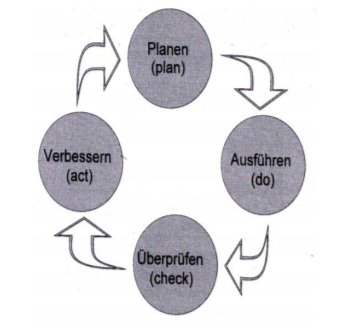
\includegraphics{./figures/pdca.png}
	\caption{ Plan-Do-Check-Act-Zyklus}
	\label{fig:pdca}
	\cite{PDCA-Zyklus}
\end{figure}

Auf dem Bild \ref{fig:pdca} wird die PDCA Zyklus dargestellte, und es ist ganz sichtbar dass die Qualitätsmethode sehr gut für die Verbesserung von Software und Programmen ist. Deshalb wurde auch diese Methode gewählt, weil durch Error und Checking konnten die Fehler gefunden, analysiert und verbessert. Das passt wirklich gut beim Team, wenn sie keine Erfahrungen mit bestimmenden Programmiersprachen bzw. Softwareprogrammen haben.
\bigbreak
Oben bei den Herausforderungen war klar, dass wenn Probleme getroffen wurden, wurden sie durch Hilfe von Tutorials bzw. Net Blogs gelost. Durch verschiedene Zyklen beachtet man auch bei den Risiken, weil wenn etwas nicht funktionier, wird schnell das Problem gefunden und später wird eine andere Losungswegen bestimmt.
 
\chapter{Ergebnisse - Jordi}
\section{Datenbank}
Für den Bereich Datenbank wurde ordentlich jede Woche programmiert, wo seit dem Anfang wurde es Recherche über verschiedenen Arten von Gesichtserkennung Datenbank, und später hat die Planung und Design von Datenbankentwurf begonnen. Es gab auch viele Änderungen abhängig von anderen Teilbereichen des Projektes. Die Datenbank musst immer geändert werden, und nach den Gesichtsdaten anpassen, damit alles in Ordnung ist.
Die folgenden Punkten der Datenbank wurden realisiert:

\begin{itemize}
	\item Datenbankdesign
	\item Erstellen von Tabellen
	\item Log Table
	\item Triggers
	\item Zugriffsrechte
\end{itemize}
Die Datenbank sollte fast fertig sein, nur kleine Anderungen konnten durchgefuhrt werden, wie fur die Backup von Daten.
\section{Tieferkennung}
Für den anderen Bereich Tieferkennung wurde gearbeitet aber nicht mit einem hohen Niveau wegen der Probleme beim Gesicht Erkennung, weil Tieferkennung ein letztes Ziel von dem Projekt ist. Hier wurde natürlich Recherche gemacht, und ein kleines stuck Programm geschrieben, nur zum Ausprobieren von Bibliothek und OpenCV.
\chapter{Evaluierung und Resümee}
\section{Wertschöpfung und Lessons Learned}
Also, nach einige Wochen sind wir zu Idee gekommen, dass die Planung eine große Rolle in diesem Projekt spielt, weil das Team must genau spezifizieren was jeder macht, und auch die wichtigsten Punkte, wie z.B der Losungsweg. Bei den nächsten Treffungen soll mehr über den Problemen diskutiert werden, damit klar für jeden was genau zu tun ist. Eine chaotische Arbeit wird keine guten Ergebnisse bringen, weil auch eine Software bzw. Programm, dass ohne Struktur geschrieben wird, wird schwierig zum Lesen und Verstehen.
